\documentclass{standalone}
\usepackage{tikz}
\usetikzlibrary{automata,positioning}

\begin{document}
  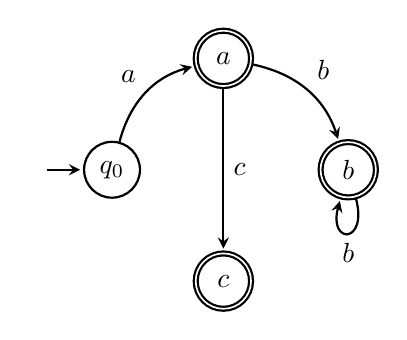
\begin{tikzpicture}[%
    >=stealth,
    shorten >=1pt,
    node distance=2cm,
    on grid,
    auto,
    state/.append style={minimum size=2em},
    thick
  ]
    \node[state, initial, initial text = {}] (A) {$q_0$};
    \node[state] (B) [accepting, above right of=A] {$a$};
    \node[state] (C) [accepting, right= 3cm of A] {$b$};
    \node[state] (D) [accepting, below right= of A] {$c$};

    \path[->]
              (A)         edge [bend left]  node {$a$} (B)
              (B)         edge [bend left] node {$b$} (C)
              (C)         edge [loop below]  node {$b$} (C)
              (B)         edge [] node {$c$} (D);
  \end{tikzpicture}
\end{document}